\begin{figure}
\begin{center}
\noindent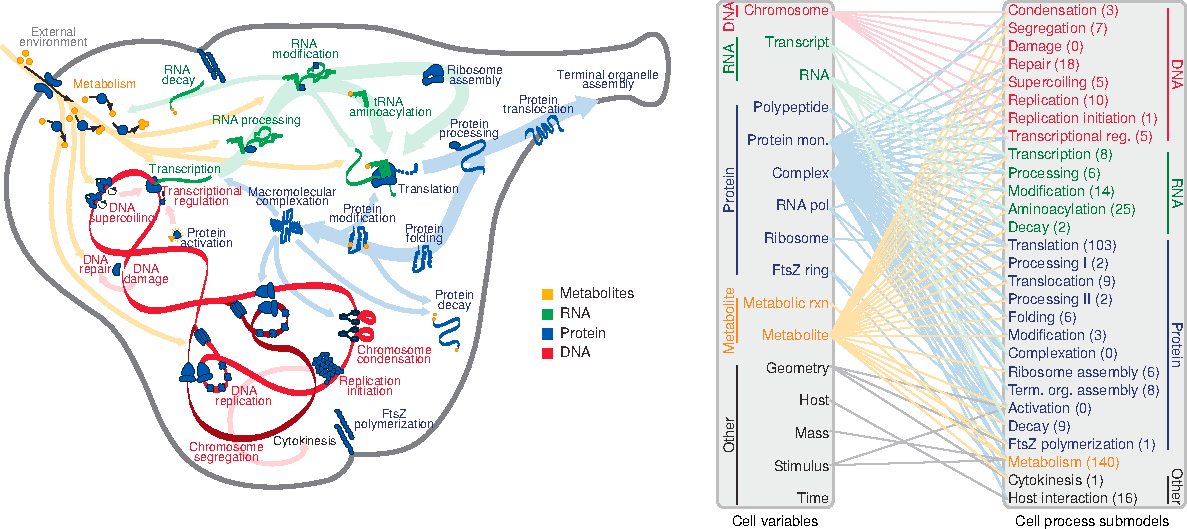
\includegraphics[width=0.8\columnwidth]{fig/cellprocessesdiagram.pdf}
\end{center}
\caption{A schematic depiction of some processes underlying a prokaryotic organism (\emph{M. genitalium}) used in developing an individual life-cycle computational model. Adapted from ref.}
\label{fig:cellprocess}
\end{figure}
Many salient features of biological organization at the level of a simple parasitic single-celled organism have recently been encapsulated in a unified computational model of the life-cycle of such a cell. In particular, this model tracks 16 important cell-level variables that each depend on a specified subset of 28 cellular processes. Figure~\ref{fig:cellprocess} shows a schematic depicting the interrelationships between these processes specified in the context of this model.

\begin{figure}
\begin{center}
\noindent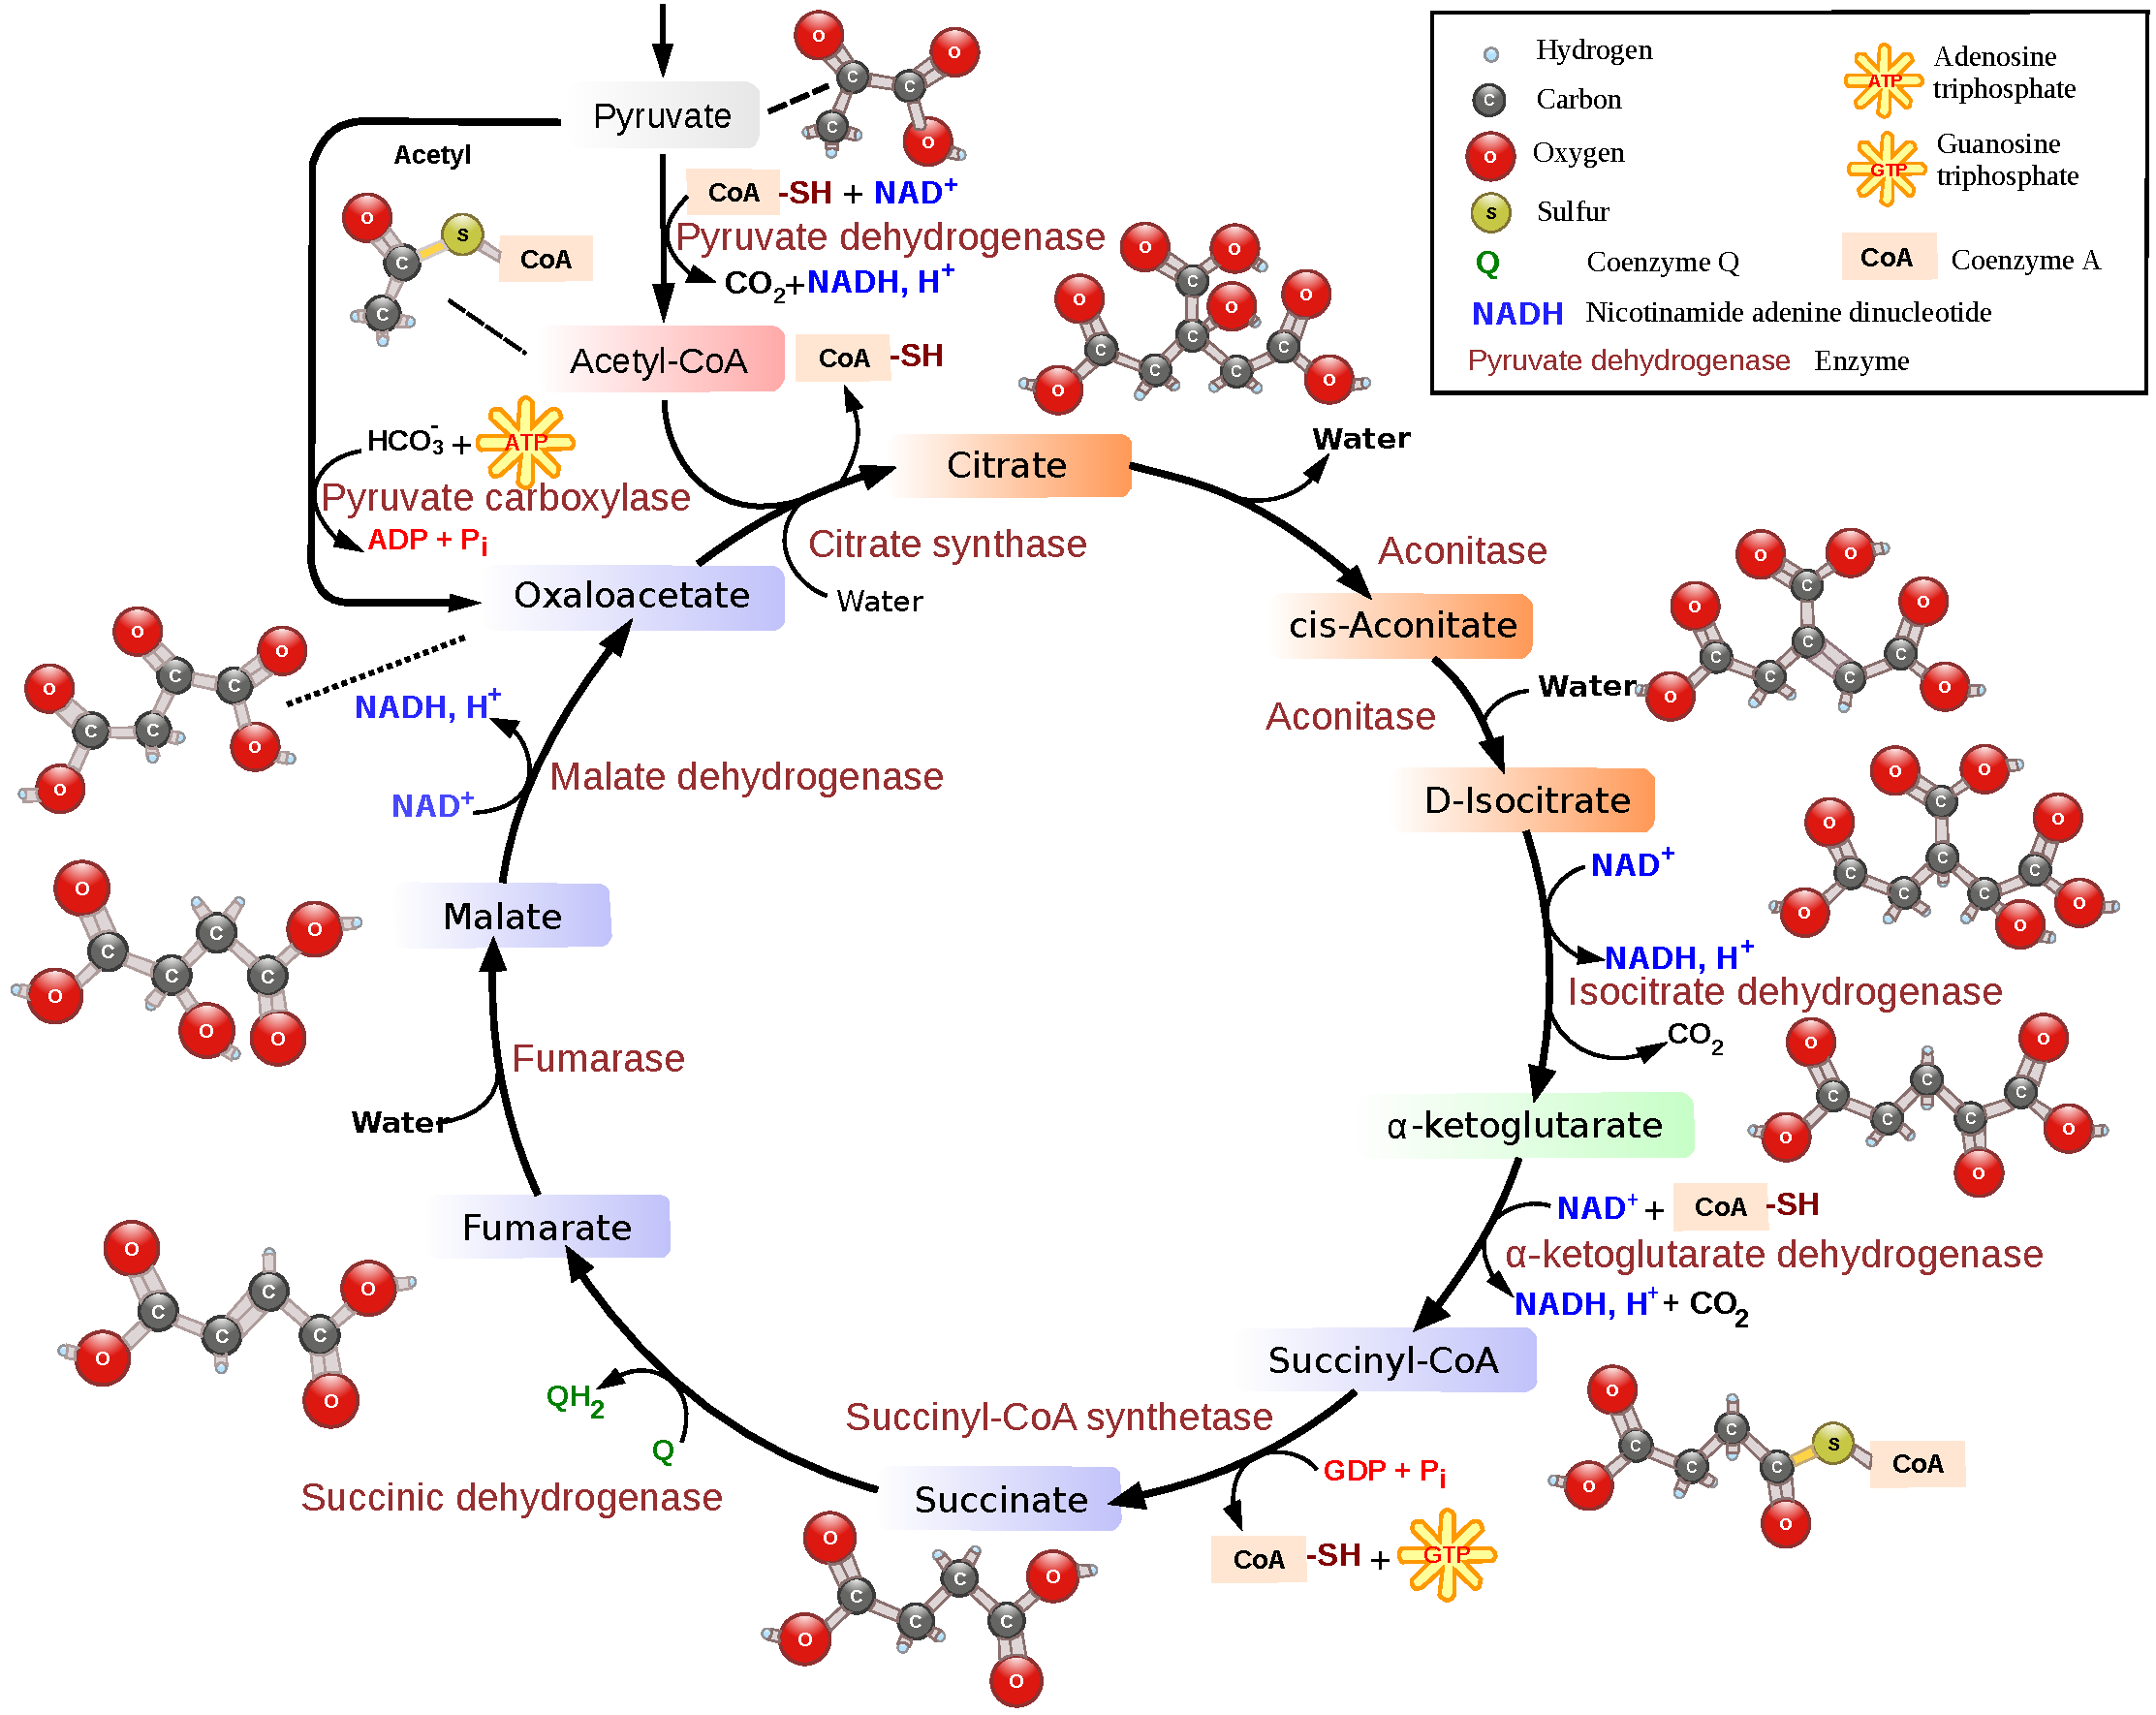
\includegraphics[width=0.5\columnwidth]{fig/Citric_acid_cycle.pdf}
\end{center}
\caption{An informal model of the citric acid cycle in terms of biochemical reactions.}
\label{fig:ctacyc}
\end{figure}
From an energetic, and thus physical, perspective, metabolic processes like the citric acid cycle (see Figure \ref{fig:ctacyc} \todo{insert adaptation reference to Karr/Covert in legend}) are certainly fundamental to the existence and persistence of all evolvable systems. As shown in Figure~\ref{fig:cellprocess}, metabolic processes form the connection between the dual components induced by considering cells as systems in the first place: the internal and the external environment. Moreover, it has been argued that metabolic processes form the basis or atomic level in a hierarchy of cellular processes. From this point of view, the complex regulatory networks involving small molecules, DNA, proteins and other molecular types are viewed as subservient to and layered atop core metabolic processes. Moreover, metabolic processes may be viewed as causally prior to the origin of evolution\todo{cite references discussing the metabolism-first view of the origin of life}.

These facts regarding the fundamental nature motivate the ability to attempt to model metabolism abstractly in attempts to characterize and parse its essential properties from those that may be no more than historical contingency. There are several existing formalisms that exist for constructing dynamical models of metabolic processes. However, these do not attempt to explain how metabolic processes originated or how they are maintained by complex networks of molecular interactions that are not themselves considered only as indirectly related to metabolic processes.

Robert Rosen suggested a formalism for metabolic networks that does attempt to abstractly incorporate the interrelationships between metabolic networks and the other regulatory networks involving interactions among DNA, RNA, and proteins\todo{citations to Rosen's original work on (M,R)-systems}. At the heart of this formalism lies the conceptual conviction that, in some sense, metabolic processes must be able to intrinsically construct at least some of their own causal antecedents. The justification for stating ``at least some of'' as opposed to all is on the basis of taking the distinction between metabolic substrate and enzyme very seriously.

In the context of a network of biochemical reactions, the heuristic distinction between metabolic substrates and enzymes is made on the basis of knowledge about the input and output of any given biochemical reaction. Those inputs that emerge from a biochemical reaction with relatively little to no change in their structure are considered to be enzymes and those whose structure is altered are considered to be substrates whose altered forms are referred to as products. 

A situation analogous to the enzyme-substrate-product abstraction \todo{this terminology is used if nowhere else in the main BioPAX publication} is formalized in a fundamental manner in type theory, category theory (see Materials and Methods) and the relationship between them. That a distinction between object and morphism was perhaps conceptually fruitful was originally suggested in Russell and Whitehead's type theory as a means of circumventing the self-referential Russell's (also known as Barber's) paradox of set theory in which one can not determine internal to the language of set theory whether a set of all sets that contain themselves contains itself or not\todo{cite Russell and Whitehead or perhaps a more modern source like John L Bell's Types, Sets and Categories}. In type theory a hierarchy is introduced that is analogous to the distinction fundamental to the definition of a category in category theory (see Materials and Methods) between objects (which are like substrates and products in terms of metabolic networks) and morphisms (which play the role of enzymes). In category theory, this distinction propagates up a hierarchy of higher-order functions where if we are in a category having a terminal, $1$, and exponential objects and we consider two objects $A$ and $B$ and morphisms between them, the collection of which is represented internal to a given category as a so-called exponential object $B^A$ or externally as $Hom(A,B)$ one of which might be $f \colon A \rightarrow B$ then the respective \emph{elements} of $A$, $B$ and $B^A$ are essentially of different types. From this perspective, while it is possible to \emph{evaluate} an element $f:B^A$ read ``an element $f$ of type $B^A$ given by $f \colon 1 \rightarrow B^A$'' at an element $a:A$ given by $a \colon 1 \rightarrow A$ to arrive at some element $b:B$ given by $b \colon 1 \rightarrow B$ it is not possible to likewise \emph{evaluate} an element $a:A$ at another element $a':A$ as this kind of statement is simply not able to be expressed within the confines of the language. If it were possible to do such a thing in some more expressive meta-language of which category theory only represents a fragment, then we can imagine that while reasoning within the language of category theory itself we have restricted ourselves to a mental state in which we are completely unaware and unable to become aware of this capacity.

The enzyme-substrate-product abstraction can be interpreted in terms of symmetric monoidal categories and depicted using corresponding string diagrams. Any metabolic reaction such as one of the first steps in the tricarboxylic acid cycle depicted in Figure \ref{fig:ctacyc} can be viewed as a morphism acting on tensored objects. The way this metaphor is constructed is to associate to a biochemical reaction such as 
$$
\text{Oxaloacetate } + \text{Acetyl CoA} + H_2O \xrightarrow[]{\text{Citrate synthase}} \text{Citrate} + \text{CoA-SH},
$$
abstract labels
$$
s_1 + s_2 + s_3 \xrightarrow[]{m_1} p_1 + p_2.
$$
This can be done for any biochemical reaction and at any level of abstraction. For example we can do the same for the net reaction that occurs for each iteration of the TCA cycle as
$$
\text{Acetyl-CoA} + 3 \text{NAD}^+ + \text{Q} + \text{GDP} + P_i + 3 H_2O \xrightarrow[]{\text{TCA cycle}} \text{CoA-SH} + 3 \text{NADH} + 3H^+ + QH_2 + \text{GTP} + 2 CO_2,
$$
where we now have to abstract from a single enzyme to the composite action of all of the enzymes directly involved in the TCA cycle to which we give the name ``TCA cycle''. The abstract labels that may be associated with this biochemical transformation are
$$
s_1 + s_2 + s_2 + s_2 + s_3 + s_4 + s_5 + s_6 + s_6 + s_6 \xrightarrow[]{f} p_1 + p_2 + p_2 + p_2 + p_3 + p_3  + p_3 + p_4 + p_5 + p_6 + p_6. 
$$
The general promiscuity of metabolic interactions in which enzymes recognize a collection of, for the most part very closely, related substrates suggests the representation of these biochemical reactions as tensor products of objects in a category. The intuition behind doing so lies in the fact that if there is a general class of substrates that can substitute for a given one, then instead of specifying a particular one, $s_1$, we should specify an entire set of them $S_1$. Then if there is another set, $S_2$ of substrates that can take the place of $s_2$, and the substrates upon which an enzyme acts is defined on $S_1 \times S_2$, then that enzyme can be said to act on any pair $(s_1,s_2)$ of substrates where $s_1 \in S_1$ and $s_2 \in S_2$. This case of viewing $S_1$ and $S_2$ as sets may come to be seen as being too restrictive in which case we would be forced to consider the abstract tensor product of two objects in a category $S_1 \otimes S_2$, which could then be specialized to a different special case than that in which $S_1$ and $S_2$ are sets. For the simple example of the Citrate synthase catalyzed aldol condensation reaction described above, we arrive at a representation in terms of a morphism in a symmetric monoidal category
\begin{eqnarray*}
m_1 \colon S_1 \otimes S_2 \otimes S_3 &\longrightarrow& P_1 \otimes P_2\\
(s_1,s_2,s_3) &\longmapsto& (p_1,p_2)
\end{eqnarray*}
The adjective ``symmetric'' is appended to monoidal category based upon the assumption that the order of combination of substrates and production of products is unimportant and thus the factors in said tensor products may be permuted. The prototype example of such a monoidal category is the category of sets with cartesian product, but the formalism is not limited to this particular representation. We will proceed thinking in terms of this particular case as a useful mental crutch for grounding intuitions, but its limitations with respect to the capacity to recognize the full generality of the formalism at hand can be severe. Indeed, we will be forced to highlight at least one case where such intuition fails in order to explain the functional closure concept.

The metabolic network formalism interpreted in symmetric monoidal categories then applies to the case in which we string together metabolic processes. An example of this is presented in Figure \ref{fig:metabolicstringdiag}. In this diagram, we have the following morphisms:
\begin{eqnarray*}
m_1 \colon S_1 \otimes S_2 &\longrightarrow& P_1 \otimes I_1,\\
m_2 \colon I_1 &\longrightarrow& P_2 \otimes I_2,\\
m_3 \colon I_2 \otimes S_3 &\longrightarrow& P_3 \otimes P_4.
\end{eqnarray*}
These morphisms can be composed as 
$$
f \cong (m_1 \circ m_2) \circ m_3 \cong m_1 \circ (m_2 \circ m_3) \cong m_1 \circ m_2 \circ m_3,
$$
where further identifying $A \cong S_1 \otimes S_2 \otimes S_3$ and $B \cong P_1 \otimes P_2 \otimes P_3 \otimes P_4$ allows us to express any metabolic network represented in the form depicted in Figure \ref{fig:metabolicstringdiag} regardless of the more or less complicated nature of intermediate interactions concisely as
$$
\xymatrix@1{
	A\ar[r]^-{f} & B.
	}
$$
In general we can consider any case of $f \colon \prod_i S_i \rightarrow \prod_j P_j$ as being denoted by $f \colon A \rightarrow B$ for $A \cong \prod_i^N S_i$ and $B \cong \prod_j^M P_j$. An element $a \colon A$ then represents a tuple $(s_1, s_2, \ldots, s_N)$ that expresses a state of metabolic input substrates and likewise for the metabolic products $b \colon B$ representing $(p_1, p_2, \ldots, p_M)$.

\begin{figure}
\begin{center}
\noindent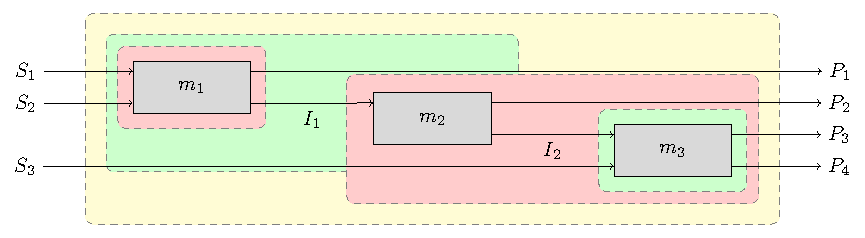
\includegraphics[width=0.9\columnwidth]{fig/blockdiagtop.pdf}
\end{center}
\caption{An abstraction of metabolic networks that can be interpreted in terms of symmetric monoidal categories.}
\label{fig:metabolicstringdiag}
\end{figure}